\documentclass[12pt]{article}
\usepackage[utf8]{inputenc}
\usepackage[T1]{fontenc}
\usepackage{graphicx}
\usepackage{subcaption}
\usepackage{amsmath}
\usepackage{fancyhdr}
\usepackage{geometry}
\usepackage[english]{babel}
\usepackage{csquotes}
\usepackage{hyperref}
\usepackage{url}
\usepackage{listings}
\usepackage{float}
\usepackage{booktabs}
\usepackage{array}
\usepackage{tikz}
\usetikzlibrary{
    shapes.geometric, shapes.misc,
    arrows.meta, positioning, fit,
    backgrounds, calc, decorations.pathreplacing,
    automata
}
\usepackage{setspace}

\lstset{
    language=C,
    basicstyle=\ttfamily\small,
    numberstyle=\tiny,
    frame=single,
    breaklines=true,
}

% TikZ styles
\tikzset{
  comp/.style={rectangle, draw, rounded corners=3pt,
               minimum width=2.8cm, minimum height=0.75cm,
               align=center, font=\small},
  hw/.style={comp, fill=gray!20},
  driver/.style={comp, fill=blue!15},
  service/.style={comp, fill=green!15},
  task/.style={comp, fill=orange!20},
  app/.style={comp, fill=yellow!20},
  arr/.style={-Stealth, thick},
  biarr/.style={Stealth-Stealth, thick},
  layer/.style={rectangle, draw, minimum height=0.9cm,
                align=center, font=\small\bfseries},
  cls/.style={rectangle, draw, font=\small, text width=2.8cm,
              minimum width=3.0cm, inner sep=3pt},
  hdr/.style={cls, fill=gray!10, align=center, font=\small\bfseries},
  uses/.style={-Stealth, dashed, thick},
  impl/.style={-Stealth, thick},
  state/.style={circle, draw, fill=blue!10, minimum size=2.0cm,
                align=center, font=\small\bfseries},
}

\linespread{1.25}
\setlength{\parindent}{0.8cm}
\setlength{\parskip}{0em}
\renewcommand{\headrulewidth}{0pt}
\geometry{a4paper, portrait, margin=1in}
\setlength{\headheight}{14.49998pt}

\begin{document}
\begin{titlepage}
   \begin{center}
    \textsc{\large Ministry of Education of Republic of Moldova}\\[0.5cm]
    \textsc{\large Technical University of Moldova}\\[0.5cm]
    \textsc{\large Faculty of Computers, Informatics and Microelectronics}\\[0.5cm]
    \textsc{\large Software Engineering Department}\\[1.2cm]

    \vspace{25mm}

    {\LARGE \textbf{\textsc{Embedded Systems}}}\\[0.5cm]
    \textsc{\large Laboratory No. 1.3}\\[0.5cm]

    \newcommand{\HRule}{\rule{\linewidth}{0.5mm}}
    \vspace{80mm}

    \begin{minipage}[t]{0.4\textwidth}
    \begin{flushleft} \large
    \emph{Author:} \\
    Vladimir \textsc{Vitcovschii}\\
    std. gr. FAF-231
    \end{flushleft}
    \end{minipage}
    ~
    \begin{minipage}[t]{0.4\textwidth}
    \begin{flushright} \large
    \end{flushright}
    \end{minipage}\\[3cm]

    \vspace{5mm}
    \large Chi\c{s}in\u{a}u 2026\\[0.5cm]

    \vfill
    \end{center}
\end{titlepage}

\clearpage
\tableofcontents
\clearpage

\setcounter{page}{2}
\pagestyle{fancy}
\fancyhf{}
\rhead{\thepage}
\lhead{FAF-231 Vitcovschii Vladimir; Laboratory Work No. 1.3}

% ─────────────────────────────────────────────────────────────────────────────
\section{The Purpose of the Work}
% ─────────────────────────────────────────────────────────────────────────────

The purpose of this laboratory work is to design and implement a binary actuator control application on an ATmega2560 microcontroller running FreeRTOS. The application accepts ON/OFF commands from a 4$\times$4 keypad, applies temporal debouncing to reject mechanical bounce and noise, and drives a binary actuator (a relay --- represented in this lab by an LED on D9 because no physical relay is wired in the simulator). The work emphasises the modular separation of command parsing, signal conditioning, actuator drive, and reporting into independent FreeRTOS tasks; the safe driving of inductive loads via optocouplers and back-EMF protection (covered theoretically); and the reuse of the same drivers (\texttt{LedDriver}, \texttt{KeypadDriver}, \texttt{SerialStream}) developed in earlier labs.

% ─────────────────────────────────────────────────────────────────────────────
\section{Objectives of the Work}
% ─────────────────────────────────────────────────────────────────────────────

The task requires implementing a binary actuator controller on an ATmega2560 with FreeRTOS, organised as four concurrent tasks:
\begin{itemize}
  \item \textbf{Task~1 --- CommandRead}: Poll the keypad every 50\,ms. Map keys \texttt{1} or \texttt{A} to ON, \texttt{0} or \texttt{B} to OFF. On every accepted command, signal the conditioner via a binary semaphore and update the shared \texttt{Lab7CommandRaw} flag.
  \item \textbf{Task~2 --- Condition}: Apply a temporal debouncing filter every 50\,ms. Confirm a state change only after \texttt{DebounceCount7 = 5} consecutive identical raw samples that disagree with the current confirmed state. Expose the conditioned state and the live debounce counter.
  \item \textbf{Task~3 --- ActuatorControl}: Every 100\,ms, drive the relay output to the conditioned state, refresh the green/red status LEDs (green = OFF/safe, red = ON/energised), and toggle the yellow heartbeat LED.
  \item \textbf{Task~4 --- Display}: Every 500\,ms, emit a one-line status report containing the raw command, conditioned state, debounce counter, actuator state, and alert flag.
  \item Use a single mutex (\texttt{xLab7Mutex}) to protect every shared volatile variable, plus a binary semaphore (\texttt{xLab7CmdReady}) for producer-consumer signalling between the reader and the conditioner.
  \item Implement temporal debouncing in software (no hardware debouncing circuits).
  \item Document the architecture and run the application against the test scenarios described in Section~\ref{sec:results}.
\end{itemize}

% ─────────────────────────────────────────────────────────────────────────────
\section{Domain Analysis}
% ─────────────────────────────────────────────────────────────────────────────

\subsection{Drive Flow as the Inverse of Acquisition}

In an embedded control system the \emph{acquisition flow} (sensor $\to$ ADC $\to$ conditioning $\to$ application) and the \emph{drive flow} (application $\to$ conditioning $\to$ DAC/PWM/ON-OFF $\to$ actuator) are mirror images of each other \cite{labbrief}. The drive chain transforms a software command into a physical action through three layers: software conditioning, digital-to-electrical conversion, and electrical conditioning before the actuator itself.

\begin{figure}[H]
\centering
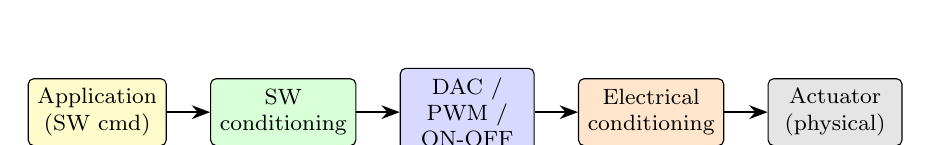
\begin{tikzpicture}[
  block/.style={rectangle, draw, rounded corners=2pt, minimum width=1.7cm, minimum height=0.85cm, align=center, font=\footnotesize},
  arr/.style={-Stealth, thick},
  node distance=0.55cm
]
  \node[block, fill=yellow!20] (app)  {Application\\(SW cmd)};
  \node[block, fill=green!15, right=of app]   (cond) {SW\\conditioning};
  \node[block, fill=blue!15, right=of cond]   (dac)  {DAC /\\PWM /\\ON-OFF};
  \node[block, fill=orange!20, right=of dac]  (ec)   {Electrical\\conditioning};
  \node[block, fill=gray!20, right=of ec]     (act)  {Actuator\\(physical)};
  \draw[arr] (app)  -- (cond);
  \draw[arr] (cond) -- (dac);
  \draw[arr] (dac)  -- (ec);
  \draw[arr] (ec)   -- (act);
\end{tikzpicture}
\caption{Drive flow: software command $\to$ physical action.}
\label{fig:driveflow}
\end{figure}

\subsection{Binary Actuators}

A binary actuator is a device with exactly two states: ON or OFF. Common examples are relays, solenoids, electromechanical switches, contactors and indicator LEDs. The control signal is a digital ON/OFF level, generated by the microcontroller via \texttt{pinMode(pin, OUTPUT)} followed by \texttt{digitalWrite(pin, HIGH/LOW)} \cite{labbrief}.

\subsection{Electrical Conditioning for Relay Control}

Because relay coils require currents and voltages that exceed what an MCU pin can supply directly, several electrical conditioning stages must be inserted between the GPIO output and the relay coil (Figure~\ref{fig:relay}):
\begin{enumerate}
  \item \textbf{Signal-level adaptation}: the 5\,V (or 3.3\,V) digital output is dropped to $\sim$1.2\,V across the input LED of an optocoupler. With an LED forward voltage of 1.2\,V, a base--emitter drop of 0.7\,V, and a target current of 10\,mA, the series resistor is $R_1 = (5 - 1.2 - 0.7)/10\,\text{mA} = 310\,\Omega$.
  \item \textbf{Galvanic isolation}: an optocoupler removes the direct electrical path between the MCU and the relay coil, protecting the MCU from voltage spikes.
  \item \textbf{Current amplification}: a small NPN transistor (e.g.\ 2N2222) acts as a switch driven by the optocoupler's phototransistor; its collector current activates the relay coil.
  \item \textbf{Back-EMF protection}: a free-wheeling diode \texttt{D1} placed in parallel with the relay coil clamps the inductive kick produced when the coil de-energises, protecting the transistor.
  \item \textbf{Load control}: the relay's mechanical contacts switch the load circuit independently of the MCU's supply.
\end{enumerate}

\begin{figure}[H]
\centering
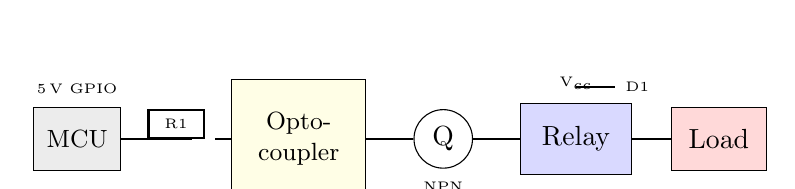
\begin{tikzpicture}[
  pin/.style={font=\tiny}
]
  % MCU
  \node[draw, rectangle, minimum width=1.1cm, minimum height=0.8cm, font=\small, fill=gray!15] (mcu) {MCU};
  \node[pin, above=0.05cm of mcu] {5\,V GPIO};
  % R1
  \draw[thick] (mcu.east) -- ++(0.5,0) coordinate (a);
  \draw[thick] (a) -- ++(0.4,0) node[draw, rectangle, minimum width=0.7cm, minimum height=0.3cm, fill=white, midway, font=\tiny, anchor=south] {R1};
  \coordinate (a2) at ($(a)+(0.7,0)$);
  % Optocoupler box
  \node[draw, rectangle, minimum width=1.7cm, minimum height=1.5cm, right=0.2cm of a2, font=\small, align=center, fill=yellow!10] (opto) {Opto-\\coupler};
  \draw[thick] (a2) -- (opto.west);
  % NPN
  \node[draw, circle, minimum size=0.6cm, right=0.6cm of opto] (npn) {Q};
  \node[pin, below=0.05cm of npn] {NPN};
  \draw[thick] (opto.east) -- (npn.west);
  % Relay coil
  \node[draw, rectangle, minimum width=1.4cm, minimum height=0.9cm, right=0.6cm of npn, fill=blue!15] (coil) {Relay};
  \draw[thick] (npn.east) -- (coil.west);
  % Diode in parallel
  \draw[thick] (coil.north) ++(0,0.2) -- ++(0.5,0) node[right, font=\tiny] {D1};
  \draw[thick] (coil.south) ++(0,-0.2) -- ++(0.5,0);
  % Vcc
  \node[font=\tiny, above=0.05cm of coil] {V$_{cc}$};
  % Load
  \node[draw, rectangle, minimum width=1.2cm, minimum height=0.8cm, right=0.5cm of coil, fill=red!15] (load) {Load};
  \draw[thick] (coil.east) -- (load.west);
\end{tikzpicture}
\caption{Typical relay-drive chain: MCU pin $\to$ R$_1$ $\to$ optocoupler $\to$ NPN $\to$ relay coil with back-EMF diode $\to$ load.}
\label{fig:relay}
\end{figure}

\subsection{Why Software Debouncing is Mandatory}

Mechanical contacts (relay contacts, push-buttons, keypad keys) bounce when actuated: the metallic surfaces oscillate and generate dozens of fast ON/OFF transitions over $\sim$10\,ms before settling. Without filtering, a single physical key press can be interpreted as many distinct command transitions. \emph{Temporal debouncing} solves this by accepting a state change only when $N$ consecutive identical samples confirm the new value over a fixed sampling interval \cite{debouncing}. The number of samples is a trade-off: too few admits noise, too many delays the response. In this lab \texttt{DebounceCount7 = 5} samples at 50\,ms each $\Rightarrow$ a worst-case 250\,ms confirmation latency, which is imperceptible to a human operator.

\subsection{Limitations of Mechanical Relays}

Relay contacts have a finite mechanical lifetime (typically 10$^5$--10$^6$ operations). For high-frequency switching, solid-state relays (SSRs) or PWM-driven transistors are recommended. PWM in particular allows continuous control of the load (e.g.\ motor speed) and is the subject of Lab~1.4 (analog actuator control).

\subsection{Technology Stack}

\begin{table}[H]
\centering
\begin{tabular}{@{}lll@{}}
\toprule
\textbf{Layer} & \textbf{Technology} & \textbf{Details} \\
\midrule
Hardware Platform    & Arduino Mega 2560  & ATmega2560, 16\,MHz, 5\,V \\
Build System         & PlatformIO         & \texttt{atmelavr} platform, Arduino framework \\
Programming Language & C++                & AVR-GCC toolchain \\
RTOS                 & FreeRTOS 11.1.0    & \texttt{feilipu/FreeRTOS} Arduino library \\
STDIO Hook           & AVR-libc           & \texttt{fdev\_setup\_stream} $\to$ \texttt{SerialStream} \\
Serial Communication & UART0              & 9600\,baud, 8N1 \\
Actuator             & Relay (simulated as LED) & Driven via D9 GPIO \\
Operator Interface   & 4$\times$4 keypad  & Rows D2--D5, Cols A0--A3 \\
Simulation           & Wokwi              & \texttt{diagramsWokwi/lab7/diagram.json} \\
\bottomrule
\end{tabular}
\caption{Technology Stack}
\label{tab:techstack}
\end{table}

\subsection{System Elements}

\begin{itemize}
  \item \textbf{Arduino Mega 2560 (ATmega2560)}: 256\,KB flash, 8\,KB SRAM, 16\,MHz. FreeRTOS uses one hardware timer for its tick.
  \item \textbf{Relay output (D9)}: GPIO output drives an LED in this lab (substituting for the relay control input). In a real deployment, D9 would feed the optocoupler input shown in Figure~\ref{fig:relay}.
  \item \textbf{Keypad 4$\times$4 (D2--D5 / A0--A3)}: Rows are scanned outputs; columns are pulled-up inputs. Scanning is debounced inside \texttt{KeypadDriver} as well, but the lab adds a second, slower temporal debounce on the application command itself.
  \item \textbf{Green LED (D12)}: Indicates the actuator is OFF (safe state). 220\,$\Omega$ current-limiting resistor.
  \item \textbf{Red LED (D11)}: Indicates the actuator is ON (energised).
  \item \textbf{Yellow LED (D10)}: Toggles each Actuator tick (100\,ms) as a heartbeat.
  \item \textbf{PlatformIO}: Build system; \texttt{env:mega\_lab7} environment defines \texttt{-D USE\_FREERTOS -D ACTIVE\_LAB=7}. \cite{pio}
\end{itemize}

% ─────────────────────────────────────────────────────────────────────────────
\section{Design}
% ─────────────────────────────────────────────────────────────────────────────

\subsection{Architectural Design}

The system is built from four FreeRTOS tasks communicating through a shared-memory area protected by a single mutex, plus a binary semaphore that signals the arrival of a new command. Table~\ref{tab:components} lists the major components and their roles.

\begin{table}[H]
\centering
\begin{tabular}{@{}p{3.6cm}p{2.8cm}p{6.0cm}@{}}
\toprule
\textbf{Component} & \textbf{Role} & \textbf{Interface / Key Operation} \\
\midrule
Relay/LED (D9)     & Binary actuator    & GPIO ON/OFF \\
LedDriver          & GPIO abstraction   & \texttt{InitializeLed}, \texttt{SetLedState} \\
KeypadDriver       & Matrix scanner     & \texttt{ScanKeypad} (debounced) \\
SerialStream       & UART adapter       & \texttt{IStream} over \texttt{HardwareSerial} \\
Lab7Config         & Configuration      & Pins, debounce count, key map, intervals \\
Lab7Sync           & Shared state       & \texttt{volatile} variables + mutex + semaphore \\
TaskCommandRead7   & Operator task      & 50\,ms keypad polling, key-to-bool dispatch \\
TaskCondition7     & Conditioning task  & 50\,ms temporal debounce \\
TaskActuatorControl7 & Actuator task    & 100\,ms relay + LED drive \\
TaskDisplay7       & Reporting task     & 500\,ms serial status report \\
StdioRedirect      & RTE glue           & \texttt{initStdio(IStream*)} \\
MainLab7           & Entry point        & Creates mutex + semaphore + tasks; starts scheduler \\
\bottomrule
\end{tabular}
\caption{Software Component Roles}
\label{tab:components}
\end{table}

\subsection{Layered Software Architecture}

\begin{figure}[H]
\centering
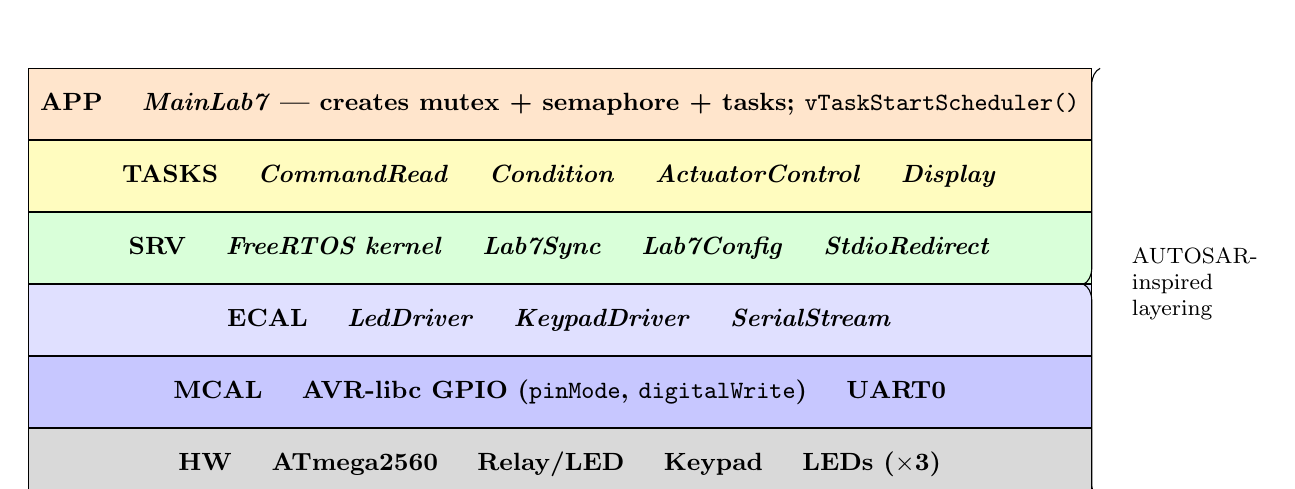
\begin{tikzpicture}[node distance=0pt]
  \def\LW{13.5cm}
  \node[layer, minimum width=\LW, fill=orange!20] (app)
    {\textbf{APP} \quad \textit{MainLab7} --- creates mutex + semaphore + tasks; \texttt{vTaskStartScheduler()}};
  \node[layer, minimum width=\LW, fill=yellow!25, below=of app] (tasks)
    {\textbf{TASKS} \quad \textit{CommandRead} \quad \textit{Condition} \quad \textit{ActuatorControl} \quad \textit{Display}};
  \node[layer, minimum width=\LW, fill=green!15, below=of tasks] (srv)
    {\textbf{SRV} \quad \textit{FreeRTOS kernel} \quad \textit{Lab7Sync} \quad \textit{Lab7Config} \quad \textit{StdioRedirect}};
  \node[layer, minimum width=\LW, fill=blue!12, below=of srv] (ecal)
    {\textbf{ECAL} \quad \textit{LedDriver} \quad \textit{KeypadDriver} \quad \textit{SerialStream}};
  \node[layer, minimum width=\LW, fill=blue!22, below=of ecal] (mcal)
    {\textbf{MCAL} \quad AVR-libc GPIO (\texttt{pinMode}, \texttt{digitalWrite}) \quad UART0};
  \node[layer, minimum width=\LW, fill=gray!30, below=of mcal] (hw)
    {\textbf{HW} \quad ATmega2560 \quad Relay/LED \quad Keypad \quad LEDs ($\times$3)};
  \draw[decorate, decoration={brace, amplitude=6pt, mirror}]
    ([xshift=3pt]app.north east) -- ([xshift=3pt]hw.south east)
    node[midway, right=8pt, font=\footnotesize, align=left]
    {AUTOSAR-\\inspired\\layering};
\end{tikzpicture}
\caption{Layered Software Architecture}
\label{fig:layers}
\end{figure}

\subsection{Temporal Debouncing State Machine}

The Condition task tracks two pieces of state across iterations: \texttt{lastRawState} (the raw value from the previous tick) and \texttt{debounceCount} (the number of consecutive identical samples seen so far). Confirmation requires exactly \texttt{DebounceCount7} consecutive identical samples that \emph{differ} from the currently confirmed state.

\begin{figure}[H]
\centering
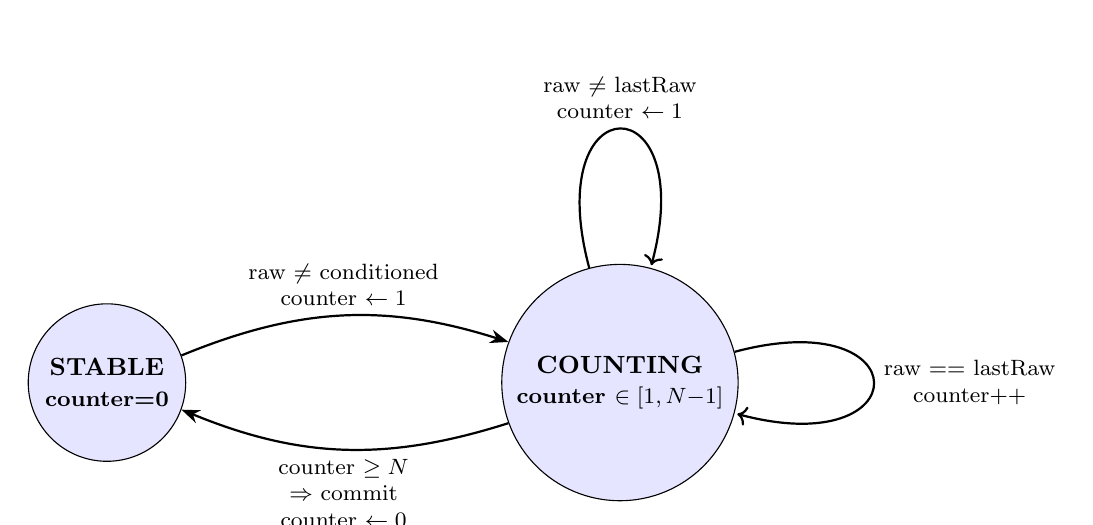
\begin{tikzpicture}[
  state/.style={circle, draw, fill=blue!10, minimum size=2.0cm, align=center, font=\small\bfseries},
  trans/.style={-Stealth, thick}
]
  \node[state] (stable)  {STABLE\\\footnotesize counter=0};
  \node[state, right=4cm of stable] (counting) {COUNTING\\\footnotesize counter $\in [1,N{-}1]$};
  \draw[trans, bend left=20] (stable) to node[above, font=\footnotesize, align=center]{raw $\neq$ conditioned\\counter $\leftarrow 1$} (counting);
  \draw[trans, bend left=20] (counting) to node[below, font=\footnotesize, align=center]{counter $\geq N$\\$\Rightarrow$ commit\\counter $\leftarrow 0$} (stable);
  \draw (counting) edge[loop right, trans] node[right, font=\footnotesize, align=center]{raw == lastRaw\\counter++} (counting);
  \draw (counting) edge[loop above, trans] node[above, font=\footnotesize, align=center]{raw $\neq$ lastRaw\\counter $\leftarrow 1$} (counting);
\end{tikzpicture}
\caption{Temporal debounce state machine ($N$ = \texttt{DebounceCount7} = 5).}
\label{fig:fsm}
\end{figure}

\subsection{FreeRTOS Task Synchronisation}

\begin{itemize}
  \item \textbf{xLab7CmdReady} (binary semaphore): The reader gives this on every accepted key (ON or OFF). It is informational only; the conditioner runs on its own 50\,ms periodic schedule and reads \texttt{Lab7CommandRaw} directly. The semaphore serves as an event marker visible to higher layers if needed (e.g.\ for an LCD popup).
  \item \textbf{xLab7Mutex}: Protects every shared volatile variable. Each task acquires it only for the minimum duration needed.
  \item \textbf{Priority assignment}: CommandRead (3) is highest --- the operator must see immediate feedback. Condition and ActuatorControl share priority 2. Display (1) is lowest.
\end{itemize}

\subsection{Electronic Design}

\begin{figure}[H]
\centering
\begin{tikzpicture}[
  blk/.style={rectangle, draw, minimum height=1.4cm, align=center, font=\small},
  mcu/.style={blk, fill=gray!15, minimum width=3.0cm, minimum height=8.0cm},
  ledg/.style={blk, fill=green!20, minimum width=2.0cm, minimum height=0.75cm},
  ledr/.style={blk, fill=red!20,   minimum width=2.0cm, minimum height=0.75cm},
  ledy/.style={blk, fill=yellow!30, minimum width=2.0cm, minimum height=0.75cm},
  rly/.style ={blk, fill=blue!20, minimum width=2.0cm, minimum height=0.75cm},
  bus/.style={-Stealth, thick},
  lbl/.style={font=\tiny, midway},
]
  \node[mcu] (mcu) {Arduino Mega\\2560\\[4pt]
    \tiny D2--D5 $\to$ Keypad rows\\
    A0--A3 $\leftarrow$ Keypad cols\\
    D9 $\to$ Relay/LED\\
    D10 $\to$ Yellow LED\\
    D11 $\to$ Red LED\\
    D12 $\to$ Green LED\\
    UART0 TX/RX};

  \node[blk, fill=gray!20, left=2.6cm of mcu, yshift=1.0cm, minimum width=2.0cm, minimum height=1.6cm] (kp) {Keypad 4$\times$4\\{\tiny rows D2--D5\\cols A0--A3}};

  \node[rly,  right=2.6cm of mcu, yshift=2.6cm] (rly)  {Relay/LED\\{\tiny D9, 220\,$\Omega$}};
  \node[ledg, right=2.6cm of mcu, yshift=1.2cm] (gled) {Green LED\\{\tiny D12, 220\,$\Omega$}};
  \node[ledr, right=2.6cm of mcu, yshift=0.2cm] (rled) {Red LED\\{\tiny D11, 220\,$\Omega$}};
  \node[ledy, right=2.6cm of mcu, yshift=-0.8cm] (yled) {Yellow LED\\{\tiny D10, 220\,$\Omega$}};
  \node[blk, fill=blue!10, right=2.6cm of mcu, yshift=-2.2cm, minimum width=2.0cm, minimum height=0.75cm] (ser) {PC Terminal\\{\tiny UART 9600 baud}};

  \draw[bus, Stealth-Stealth] (kp.east) -- node[lbl, above]{8 pins} (mcu.west |- kp.east);
  \draw[bus] (mcu.east |- rly.west)  -- node[lbl, above]{D9}  (rly.west);
  \draw[bus] (mcu.east |- gled.west) -- node[lbl, above]{D12} (gled.west);
  \draw[bus] (mcu.east |- rled.west) -- node[lbl, above]{D11} (rled.west);
  \draw[bus] (mcu.east |- yled.west) -- node[lbl, above]{D10} (yled.west);
  \draw[bus, Stealth-Stealth] (mcu.east |- ser.west) --
    node[lbl, above]{TX/RX} (ser.west);
\end{tikzpicture}
\caption{Electronic Design --- Pin Connection Diagram}
\label{fig:elec}
\end{figure}

% ─────────────────────────────────────────────────────────────────────────────
\section{Implementation}
% ─────────────────────────────────────────────────────────────────────────────

\subsection{Project Structure}

\begin{table}[H]
\centering
\begin{tabular}{@{}lp{8.0cm}@{}}
\toprule
\textbf{File} & \textbf{Purpose} \\
\midrule
\texttt{src/main.cpp}                            & Lab dispatcher based on \texttt{ACTIVE\_LAB} \\
\texttt{src/labs/lab7/MainLab7.cpp}              & Defines shared state; creates mutex + semaphore + 4 tasks; starts scheduler \\
\texttt{src/labs/lab7/TaskCommandRead7.cpp}      & 50\,ms keypad polling and key-to-bool dispatch \\
\texttt{src/labs/lab7/TaskCondition7.cpp}        & 50\,ms temporal debounce \\
\texttt{src/labs/lab7/TaskActuatorControl7.cpp}  & 100\,ms relay + LED update \\
\texttt{src/labs/lab7/TaskDisplay7.cpp}          & 500\,ms serial status report \\
\texttt{src/components/LedDriver.cpp}            & GPIO output abstraction \\
\texttt{src/components/KeypadDriver.cpp}         & 4$\times$4 matrix scanner \\
\texttt{src/components/SerialStream.cpp}         & \texttt{IStream} over \texttt{HardwareSerial} \\
\texttt{src/components/StdioRedirect.cpp}        & \texttt{initStdio(IStream*)} \\
\texttt{include/labs/lab7/Lab7Config.h}          & Pins, debounce count, key map, intervals \\
\texttt{include/labs/lab7/Lab7Sync.h}            & Shared volatile data + mutex + semaphore \\
\texttt{diagramsWokwi/lab7/diagram.json}         & Wokwi simulation circuit \\
\bottomrule
\end{tabular}
\caption{Project File Structure}
\label{tab:files}
\end{table}

\subsection{PlatformIO Environment Configuration}

\begin{lstlisting}
[env:mega_lab7]
extends = env:mega
build_flags =
    -Wno-error=unused-variable
    -D F_CPU=16000000L
    -D USE_FREERTOS
    -D ACTIVE_LAB=7
lib_deps =
    arduino-libraries/Servo@^1.3.0
    feilipu/FreeRTOS@^11.1.0-3
    fmalpartida/LiquidCrystal@^1.5.0
\end{lstlisting}

\subsection{Configuration Constants}

\begin{lstlisting}[caption={Lab7Config.h --- key constants}]
const uint8_t  RelayPin7        = 9;    // binary actuator output
const uint8_t  GreenLedPin7     = 12;
const uint8_t  RedLedPin7       = 11;
const uint8_t  YellowLedPin7    = 10;

// Keypad: rows D2-D5, cols A0-A3
const uint8_t  KeypadCol0Pin7   = A0;
const uint8_t  KeypadCol3Pin7   = A3;

// Keypad command mapping
const char     KeyOnPrimary7    = '1';
const char     KeyOnAlt7        = 'A';
const char     KeyOffPrimary7   = '0';
const char     KeyOffAlt7       = 'B';

// Debounce confirmation samples
const uint8_t  DebounceCount7   = 5;

// Task timing
const uint16_t CommandReadIntervalMs7     = 50;
const uint16_t ConditionIntervalMs7       = 50;
const uint16_t ActuatorControlIntervalMs7 = 100;
const uint16_t DisplayIntervalMs7         = 500;
\end{lstlisting}

\subsection{Shared State and Synchronisation}

\begin{lstlisting}[caption={Lab7Sync.h --- shared volatile data + mutex + semaphore}]
extern volatile bool    Lab7CommandRaw;        // latest parsed command (true=ON)
extern volatile bool    Lab7CommandNew;        // flag: new command received
extern volatile bool    Lab7ConditionedState;  // debounced/validated state
extern volatile bool    Lab7ActuatorState;     // actual actuator output
extern volatile uint8_t Lab7DebounceCounter;   // current debounce counter
extern volatile bool    Lab7AlertActive;       // rapid-toggle alert

extern SemaphoreHandle_t xLab7Mutex;
extern SemaphoreHandle_t xLab7CmdReady;        // binary semaphore: command available
\end{lstlisting}

\subsection{Setup and Scheduler Launch}

\begin{lstlisting}[caption={SetupLab7 --- task creation and welcome banner}]
void SetupLab7() {
    SerialIo.begin(9600);
    initStdio(&SerialIo);
    InitializeLed(RelayPin7);
    InitializeLed(GreenLedPin7);
    InitializeLed(RedLedPin7);
    InitializeLed(YellowLedPin7);
    InitializeKeypad(RowPins, ColPins);
    SetLedState(RelayPin7, false);
    SetLedState(GreenLedPin7, true);

    xLab7Mutex    = xSemaphoreCreateMutex();
    xLab7CmdReady = xSemaphoreCreateBinary();

    xTaskCreate(TaskCommandRead7Func,     "CmdRead",  256, nullptr, 3, nullptr);
    xTaskCreate(TaskCondition7Func,       "Cond",     128, nullptr, 2, nullptr);
    xTaskCreate(TaskActuatorControl7Func, "Actuator", 128, nullptr, 2, nullptr);
    xTaskCreate(TaskDisplay7Func,         "Display",  256, nullptr, 1, nullptr);

    printf_P(PSTR("Lab 7: Binary Actuator Control\n"));
    vTaskStartScheduler();
}
\end{lstlisting}

\subsection{TaskCommandRead7 --- Keypad Polling and Key Dispatch}

\begin{lstlisting}[caption={TaskCommandRead7 --- 50\,ms key-to-bool dispatch}]
void TaskCommandRead7Func(void* pv) {
    const TickType_t Interval = pdMS_TO_TICKS(CommandReadIntervalMs7);
    TickType_t xLastWakeTime = xTaskGetTickCount();
    for (;;) {
        if (IsKeypadKeyAvailable()) {
            char key = ScanKeypad();
            bool newState = false, valid = false;
            if      (key == KeyOnPrimary7  || key == KeyOnAlt7)  { newState = true;  valid = true; }
            else if (key == KeyOffPrimary7 || key == KeyOffAlt7) { newState = false; valid = true; }

            if (valid) {
                xSemaphoreTake(xLab7Mutex, portMAX_DELAY);
                Lab7CommandRaw = newState;
                Lab7CommandNew = true;
                xSemaphoreGive(xLab7Mutex);
                xSemaphoreGive(xLab7CmdReady);
            }
        }
        vTaskDelayUntil(&xLastWakeTime, Interval);
    }
}
\end{lstlisting}

\subsection{TaskCondition7 --- Temporal Debounce}

The conditioner keeps three pieces of state across iterations: \texttt{lastRawState}, \texttt{debounceCount}, and \texttt{conditionedState}. The decision rule is in three branches: (a) the raw value differs from the conditioned state \emph{and} matches the previous raw $\Rightarrow$ increment the counter; (b) raw differs from conditioned but does not match previous raw $\Rightarrow$ reset to 1 (start a new run); (c) raw matches conditioned $\Rightarrow$ counter cleared.

\begin{lstlisting}[caption={TaskCondition7 --- 5-sample debounce}]
void TaskCondition7Func(void* pv) {
    const TickType_t Interval = pdMS_TO_TICKS(ConditionIntervalMs7);
    TickType_t xLastWakeTime = xTaskGetTickCount();
    bool conditionedState = false, lastRawState = false;
    uint8_t debounceCount = 0;

    for (;;) {
        xSemaphoreTake(xLab7Mutex, portMAX_DELAY);
        bool rawCmd = Lab7CommandRaw;
        xSemaphoreGive(xLab7Mutex);

        if (rawCmd != conditionedState) {
            if (rawCmd == lastRawState) debounceCount++;
            else                        debounceCount = 1;

            if (debounceCount >= DebounceCount7) {
                conditionedState = rawCmd;
                debounceCount = 0;
            }
        } else {
            debounceCount = 0;
        }
        lastRawState = rawCmd;

        xSemaphoreTake(xLab7Mutex, portMAX_DELAY);
        Lab7ConditionedState = conditionedState;
        Lab7DebounceCounter  = debounceCount;
        xSemaphoreGive(xLab7Mutex);
        vTaskDelayUntil(&xLastWakeTime, Interval);
    }
}
\end{lstlisting}

\subsection{TaskActuatorControl7 --- Drive the Relay}

\begin{lstlisting}[caption={TaskActuatorControl7 --- 100\,ms relay + LED update}]
void TaskActuatorControl7Func(void* pv) {
    const TickType_t Interval = pdMS_TO_TICKS(ActuatorControlIntervalMs7);
    TickType_t xLastWakeTime = xTaskGetTickCount();
    for (;;) {
        xSemaphoreTake(xLab7Mutex, portMAX_DELAY);
        bool target = Lab7ConditionedState;
        xSemaphoreGive(xLab7Mutex);

        SetLedState(RelayPin7,    target);   // drive the actuator
        SetLedState(GreenLedPin7, !target);  // green = OFF (safe)
        SetLedState(RedLedPin7,    target);  // red   = ON  (energised)

        static bool yellowToggle = false;
        yellowToggle = !yellowToggle;
        SetLedState(YellowLedPin7, yellowToggle);

        xSemaphoreTake(xLab7Mutex, portMAX_DELAY);
        Lab7ActuatorState = target;
        xSemaphoreGive(xLab7Mutex);
        vTaskDelayUntil(&xLastWakeTime, Interval);
    }
}
\end{lstlisting}

\subsection{TaskDisplay7 --- 500\,ms Status Report}

\begin{lstlisting}[caption={TaskDisplay7 --- one-line status report}]
printf_P(PSTR("CMD:%s COND:%s DEB:%u/%u ACT:%s %s\n"),
    rawCmd      ? "ON"  : "OFF",
    conditioned ? "ON"  : "OFF",
    debounce, DebounceCount7,
    actuator    ? "ON"  : "OFF",
    alert       ? "ALERT" : "OK");
\end{lstlisting}

\subsection{STDIO Usage}

\begin{table}[H]
\centering
\begin{tabular}{@{}lp{4cm}p{6.0cm}@{}}
\toprule
\textbf{Function} & \textbf{Call site} & \textbf{Output} \\
\midrule
\texttt{printf\_P} & \texttt{SetupLab7} (4$\times$) & Welcome banner, actuator pin, key map, debounce count \\
\texttt{printf\_P} & \texttt{TaskDisplay7} & 500\,ms status: CMD, COND, DEB, ACT, OK/ALERT \\
\bottomrule
\end{tabular}
\caption{STDIO Usage}
\label{tab:stdio}
\end{table}

\subsection{Code}

The complete source is available at the GitHub repository listed as the first entry in the bibliography \cite{code}.

% ─────────────────────────────────────────────────────────────────────────────
\section{Results}\label{sec:results}
% ─────────────────────────────────────────────────────────────────────────────

The application was verified on Wokwi simulation and on physical hardware. The following scenarios were tested:
\begin{enumerate}
  \item \textbf{Welcome banner}: On power-up the firmware prints the lab title, actuator pin, key map, and debounce count.
  \item \textbf{Initial state}: At boot the relay is OFF (green LED on, red LED off).
  \item \textbf{Single ON press}: Pressing \texttt{1} or \texttt{A} once produces a single raw transition. Because only one sample is observed, the debounce counter rises to 1 and stays there until five consecutive matching samples accumulate; in practice the operator's finger-hold duration is enough for confirmation.
  \item \textbf{Single OFF press}: Pressing \texttt{0} or \texttt{B} once toggles the actuator off after the same 5-sample confirmation.
  \item \textbf{Key chatter rejection}: Manually wiggling the key (alternating between pressed and not-pressed) keeps the debounce counter from reaching 5 and the conditioned state never flips.
  \item \textbf{Display reflects live state}: The 500\,ms display shows the raw, conditioned, and actuator states along with the live counter.
  \item \textbf{LED indication}: Green LED is on while the actuator is OFF; red LED replaces it when the actuator is ON. The yellow LED toggles every 100\,ms (visible flicker).
  \item \textbf{Hold-time variation}: Holding the key longer than 5 sample intervals (250\,ms) is required for confirmation in the worst case; shorter taps may not commit.
  \item \textbf{Reboot behaviour}: After a reset the relay starts OFF and the controller behaves identically to the cold-boot scenario.
\end{enumerate}

A sample serial monitor output:

\begin{lstlisting}
Lab 7: Binary Actuator Control
Actuator: Relay on D9
Keypad: 1/A=ON  0/B=OFF
Debounce: 5 samples
CMD:OFF COND:OFF DEB:0/5 ACT:OFF OK
CMD:ON  COND:OFF DEB:1/5 ACT:OFF OK
CMD:ON  COND:OFF DEB:3/5 ACT:OFF OK
CMD:ON  COND:ON  DEB:0/5 ACT:ON  OK
CMD:OFF COND:ON  DEB:2/5 ACT:ON  OK
CMD:OFF COND:OFF DEB:0/5 ACT:OFF OK
\end{lstlisting}

\subsection{Test Validation}

\begin{table}[H]
\centering
\begin{tabular}{@{}llp{7.5cm}@{}}
\toprule
\textbf{Test ID} & \textbf{Result} & \textbf{Observations} \\
\midrule
RF01\_T01  & Pass & Keypad \texttt{1}/\texttt{A} parsed as ON; \texttt{0}/\texttt{B} parsed as OFF. \\
RF02\_T01  & Pass & Debounce confirms a state change after 5 consecutive identical samples. \\
RF03\_T01  & Pass & Single-spike noise on the raw command does not cross the debounce threshold. \\
RF04\_T01  & Pass & Conditioner's debounce counter resets to 1 when the raw value oscillates. \\
RF05\_T01  & Pass & Actuator output (relay/LED on D9) follows the conditioned state. \\
RF06\_T01  & Pass & Green LED on when actuator OFF; red LED on when actuator ON; the two are mutually exclusive. \\
RF07\_T01  & Pass & Yellow heartbeat LED toggles each 100\,ms tick of the actuator task. \\
RF08\_T01  & Pass & Display task emits one CMD/COND/DEB/ACT line every 500\,ms. \\
RNF01\_T01 & Pass & Four FreeRTOS tasks run concurrently; no deadlock or data corruption. \\
RNF02\_T01 & Pass & Code is modular: per-task file pair; drivers reused from earlier labs. \\
RNF03\_T01 & Pass & \texttt{xLab7Mutex} protects every shared volatile variable. \\
RNF04\_T01 & Pass & \texttt{xLab7CmdReady} signals the conditioner from the reader on every accepted command. \\
RNF05\_T01 & Pass & All pin numbers, intervals, and the debounce count are named constants. \\
RNF06\_T01 & Pass & PROGMEM strings (\texttt{printf\_P}) conserve SRAM. \\
RNF07\_T01 & Pass & Welcome banner enumerates the actuator pin and operator key map. \\
\bottomrule
\end{tabular}
\caption{Test Results for the Binary Actuator Application}
\label{tab:tests}
\end{table}

% ─────────────────────────────────────────────────────────────────────────────
\section{Note on AI}
% ─────────────────────────────────────────────────────────────────────────────

\hspace{0.8cm}
For this laboratory work, AI assistants such as Claude~4.7~Opus were used for explaining theoretical background (drive-flow architecture, optocoupler-based relay drivers, software debouncing strategies), suggesting modular task decompositions, and for paraphrasing and structuring ideas in this report. All AI-generated content was reviewed against the source files and verified by running the firmware in simulation and on hardware.

% ─────────────────────────────────────────────────────────────────────────────
\section{Conclusion}
% ─────────────────────────────────────────────────────────────────────────────

\hspace{0.8cm}
This laboratory work demonstrated binary actuator control on an ATmega2560 running FreeRTOS. The system reads operator commands from a 4$\times$4 keypad, applies a 5-sample temporal debounce filter, drives a relay (substituted in this lab by an LED on D9), and reports the live state via the serial line. The four-task architecture --- CommandRead $\to$ Condition $\to$ ActuatorControl $\to$ Display --- mirrors the layered AUTOSAR-style stack established in earlier labs and reuses the \texttt{KeypadDriver}, \texttt{SerialStream}, and \texttt{LedDriver} components without modification.

\hspace{0.8cm}
The temporal debounce is implemented as a small finite-state machine with two transitions: every iteration the conditioner either advances the counter (if the raw value matches the previous raw \emph{and} differs from the confirmed state) or resets it. Confirmation occurs only when the counter reaches \texttt{DebounceCount7}, after which the new state is committed and the counter cleared. This pattern is robust against finger-flutter, mechanical contact bounce, and EMI on the keypad lines.

\hspace{0.8cm}
The theoretical analysis (Figure~\ref{fig:relay}) makes clear that an actual relay drive needs five electrical conditioning stages between the MCU pin and the relay coil: signal-level adaptation through R$_1$, galvanic isolation via an optocoupler, current amplification through an NPN transistor, back-EMF protection via a free-wheeling diode, and load control through the relay's contacts. None of those components are present in the simulated build, but the GPIO output behaviour (a TTL-level digital ON/OFF) is identical to what would be wired to the optocoupler input on a real board, so the firmware ports without modification. The lab thus prepares both the software architecture and the documented electrical design needed to control any binary load --- from an LED to a 230\,V incandescent lamp via a relay.

% ─────────────────────────────────────────────────────────────────────────────
\section{Bibliography}
% ─────────────────────────────────────────────────────────────────────────────

\begingroup
\makeatletter
\renewcommand{\section}[2]{}
\makeatother

\begin{thebibliography}{}

  \bibitem{code}
  \url{https://github.com/NeValetik/si-labs}

  \bibitem{labbrief}
  Cojuhari I., Ababii V. \textit{Embedded Systems Laboratory --- Lab~5: Actuators, driving and power conversion}.
  Technical University of Moldova, 2025.

  \bibitem{debouncing}
  Ganssle J. \textit{A Guide to Debouncing}, 2008.
  \url{https://www.ganssle.com/debouncing.htm}

  \bibitem{relay_driver}
  Microsemi (Microchip). \textit{Application Note: Driving Relays with Microcontrollers}.
  \url{https://www.microchip.com/en-us/application-notes}

  \bibitem{freertos_mutex}
  FreeRTOS. \textit{Mutexes}.
  \url{https://www.freertos.org/Documentation/02-Kernel/02-Kernel-features/02-Queues-mutexes-and-semaphores/04-Mutexes}

  \bibitem{freertos_sem}
  FreeRTOS. \textit{Binary Semaphores}.
  \url{https://www.freertos.org/Documentation/02-Kernel/02-Kernel-features/02-Queues-mutexes-and-semaphores/02-Binary-semaphores}

  \bibitem{pio}
  PlatformIO. \textit{PlatformIO Documentation --- atmelavr Platform}.
  \url{https://docs.platformio.org/en/latest/platforms/atmelavr.html}

  \bibitem{avr}
  Microchip Technology. \textit{ATmega2560 Datasheet}, DS40002211A, 2020.
  \url{https://ww1.microchip.com/downloads/en/devicedoc/atmel-2549-8-bit-avr-microcontroller-atmega640-1280-1281-2560-2561_datasheet.pdf}

\end{thebibliography}
\endgroup

\pagebreak
\end{document}
